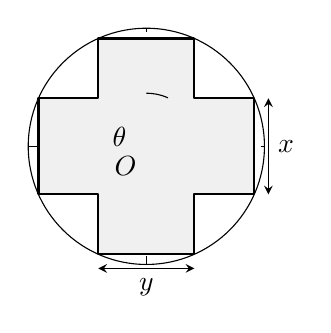
\begin{tikzpicture}[>=stealth, scale=1.5, line join=round]
  \def\th{24}
  \pgfmathsetmacro{\xh}{sin(\th)}
  \pgfmathsetmacro{\yh}{cos(\th)}
  % 圆（直径 1，图中按比例放大）
  \draw (0,0) circle (1);
  \draw[dashed] (-1,0) -- (1,0);
  \draw[dashed] (0,-1) -- (0,1);
  % 十字形
  \draw[thick, fill=gray!12]
    (\yh,\xh) -- (\xh,\xh) -- (\xh,\yh) -- (-\xh,\yh) -- (-\xh,\xh) -- (-\yh,\xh)
    -- (-\yh,-\xh) -- (-\xh,-\xh) -- (-\xh,-\yh) -- (\xh,-\yh) -- (\xh,-\xh) -- (\yh,-\xh) -- cycle;
  % 角 theta
  \draw (0,0.45) arc (90:90-\th:0.45);
  \node at ({0.40*cos(90-\th/2+90)},{0.40*sin(90-\th/2+90)}) [right=1pt] {$\theta$};
  % 尺寸标注
  \draw[<->] (\yh+0.12,-\xh) -- (\yh+0.12,\xh) node[midway,right] {$x$};
  \draw[<->] (-\xh,-\yh-0.12) -- (\xh,-\yh-0.12) node[midway,below] {$y$};
  \node[below left] at (0,0) {$O$};
\end{tikzpicture}
